\documentclass[../../main.tex]{subfiles}

\begin{document}

\section{One-Time Pad (OTP)}
OTP adalah satu-satunya algoritma kriptografi yang terbukti aman sempurna (\textit{perfect secrecy}). Ditemukan Gilbert Vernam pada 1917 dan dibuktikan Shannon pada 1949, OTP menyempurnakan Vigen\`ere Cipher dengan menghilangkan perulangan kunci periodik yang menjadi celah metode Kasiski.

\subsection{Prinsip Kerja}
Pada OTP, kunci dibangkitkan secara acak sejati dan panjangnya sama dengan panjang plainteks:
\[ |K| = |P| \]
Kunci tidak diulang: setiap bit (atau huruf) plainteks dienkripsi dengan bit kunci yang berbeda. Karena itu aturan enkripsi sama seperti Vigen\`ere, tetapi tanpa periode kunci:
\[ C_i = P_i \oplus K_i \quad\text{(biner)}\qquad\text{atau}\qquad C_i = (P_i + K_i)\bmod 26 \]
\[ P_i = C_i \oplus K_i \qquad\qquad\qquad\qquad P_i = (C_i - K_i)\bmod 26 \]
Enkripsi dan dekripsi identik karena XOR bersifat invers terhadap dirinya sendiri. Selama panjang kunci mengikuti panjang pesan, tidak ada pengulangan pola yang dapat dimanfaatkan kriptanalis. Contoh terhitung singkat diberikan pada bagian Contoh Terhitung.

\begin{figure}[htbp]
    \centering
    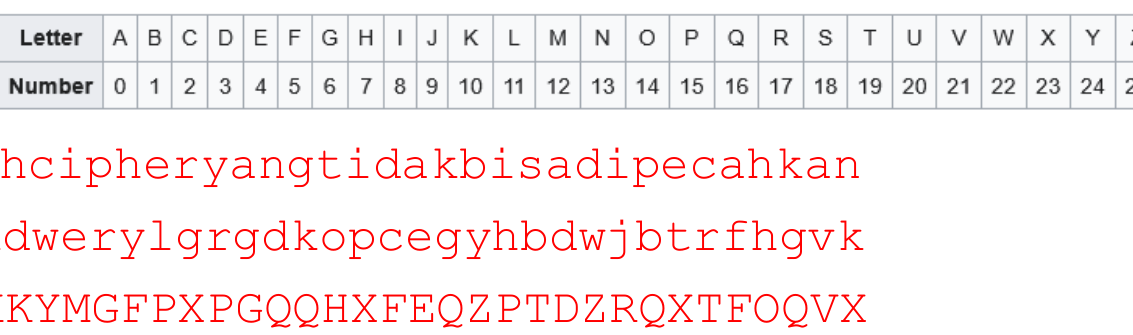
\includegraphics[width=0.8\linewidth, height=0.4\textheight, keepaspectratio]{figures/contoh-one-time-pad.png}
    \caption{Tabel konversi huruf ke angka ($A=0$ sampai $Z=25$) dan contoh enkripsi One-Time Pad: plainteks, kunci acak sepanjang pesan, serta cipherteks hasil $C=(P+K)\bmod 26$}
    \label{fig:contoh-one-time-pad}
    \sumber{Munir, \textit{IF4020 Kriptografi}, ITB.}
\end{figure}

Sebagaimana ditunjukkan Gambar~\ref{fig:contoh-one-time-pad}, cipherteks OTP tampak acak karena penjumlahan modulo 26 dengan kunci acak menyembunyikan seluruh struktur statistik plainteks.

\subsection{Kerahasiaan Sempurna}
Shannon (1949) merumuskan \textit{perfect secrecy}: pengamatan cipherteks tidak menambah informasi apa pun tentang plainteks, sehingga probabilitas posterior sama dengan probabilitas prior.
\[ P(P=p \mid C=c) = P(P=p) \]
Untuk sembarang pasangan plainteks dan cipherteks hanya ada tepat satu kunci yang memetakannya ($C=(P+K)\bmod 26$ adalah pemetaan satu-ke-satu). Akibatnya setiap plainteks yang mungkin tetap sama masuk akal di mata penyerang. \important{Kerahasiaan sempurna hanya berlaku jika tiga syarat dipenuhi: kunci benar-benar acak sejati, panjang kunci sama dengan panjang plainteks, dan kunci tidak pernah dipakai ulang.}

\subsection{Kelemahan Praktis}
Meskipun aman secara teoretis, OTP jarang dipakai karena:
\begin{itemize}
    \item Panjang kunci sama dengan panjang pesan, sehingga pesan panjang atau komunikasi berkelanjutan menuntut pembangkitan dan penyimpanan kunci acak dalam jumlah sangat besar.
    \item Pengirim dan penerima harus berbagi kunci acak yang sama; kunci acak sejati tidak dapat dibangkitkan serentak oleh keduanya tanpa saluran distribusi yang aman.
    \item Pemakaian ulang kunci (\textit{two-time pad}) berakibat fatal: untuk dua pesan berlaku $C_1\oplus C_2=P_1\oplus P_2$, sehingga XOR dua plainteks terbuka tanpa perlu mengetahui kunci.
\end{itemize}
Contoh historisnya adalah \textit{hotline} Moskow--Washington (1963) pasca Krisis Rudal Kuba, yang menggunakan perangkat OTP \textit{ITT Intelex Teletype L015}; pita kunci acaknya diterbangkan bolak-balik antara Washington DC dan Moskow.

\end{document}
